\section{Flow schema of the tool}

The data in the tool flows in several directions. User's action triggers changes in the source files. These changes cause the \texttt{TextDocumentChangeEvent} \cite{VSCodeAPI} events to be emitted. It is important to note here that the only changes that are tracked internally by VSCode are those associated with the files opened in the editor. Presumably, the reasons behind this mechanism are mainly performance ones. These events are then captured by the internal system. The internal system serves a few purposes (which are described in more detail in the subsection \ref{subsec:internal_system}). It is responsible for saving the data in the file system, compressing the data and sending it to the cloud storage (Dropbox in my case), as well as controlling the functions of the dashboard.

\begin{figure}[ht]
  \centering
  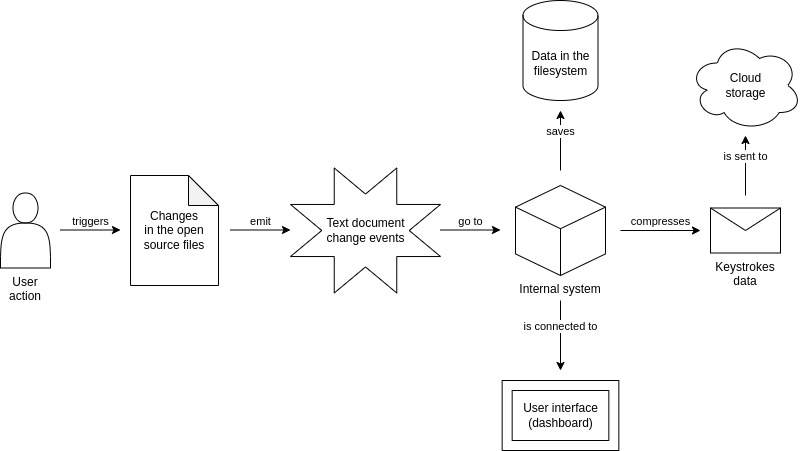
\includegraphics[scale=0.5]{chapters/methodology/graphics/coding-process-tracker.png}
  \caption{Flow schema of the tool}
\end{figure}
